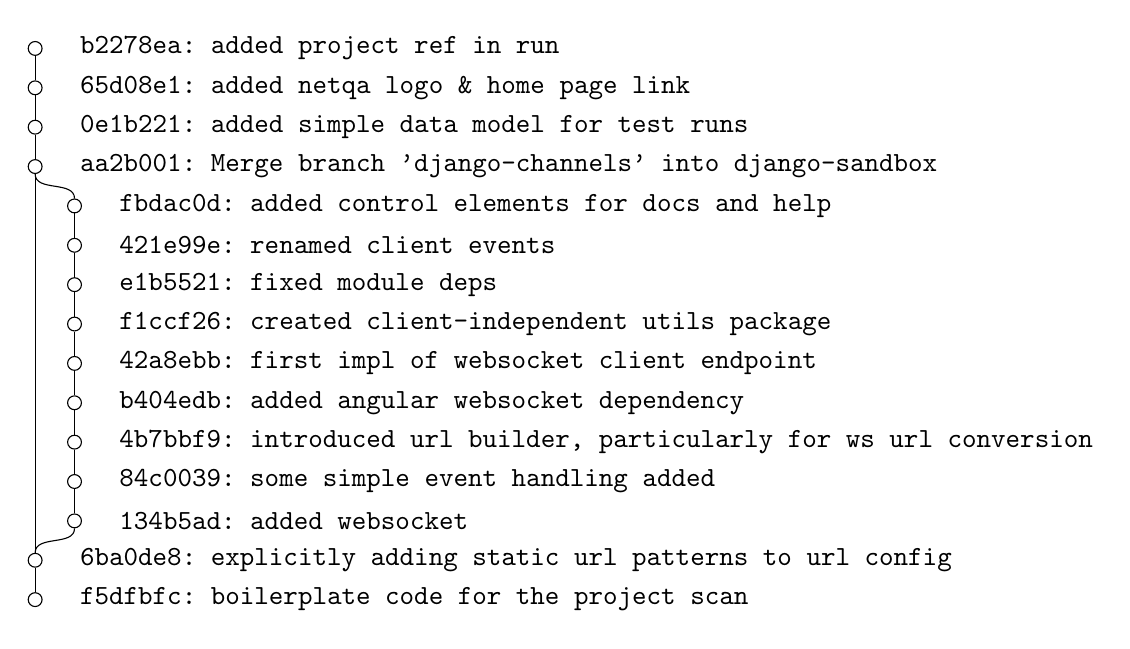
\begin{tikzpicture}
\tikzstyle{commit}=[draw,circle,fill=white,inner sep=0pt,minimum size=5pt]
\tikzstyle{every path}=[draw]

\node[commit] (b2278ea) at (0.0,-15.0) {};
\node[right,xshift=10] (label_b2278ea) at (b2278ea.east) {\verb!b2278ea: added project ref in run!};
\node[commit] (65d08e1) at (0.0,-15.5) {};
\node[right,xshift=10] (label_65d08e1) at (65d08e1.east) {\verb!65d08e1: added netqa logo & home page link!};
\path (65d08e1) to[out=90,in=-90] (b2278ea);
\node[commit] (0e1b221) at (0.0,-16.0) {};
\node[right,xshift=10] (label_0e1b221) at (0e1b221.east) {\verb!0e1b221: added simple data model for test runs!};
\path (0e1b221) to[out=90,in=-90] (65d08e1);
\node[commit] (aa2b001) at (0.0,-16.5) {};
\node[right,xshift=10] (label_aa2b001) at (aa2b001.east) {\verb!aa2b001: Merge branch 'django-channels' into django-sandbox!};
\path (aa2b001) to[out=90,in=-90] (0e1b221);
\node[commit] (fbdac0d) at (0.5,-17.0) {};
\node[right,xshift=10] (label_fbdac0d) at (fbdac0d.east) {\verb!fbdac0d: added control elements for docs and help!};
\path (fbdac0d) to[out=90,in=-90] (aa2b001);
\node[commit] (421e99e) at (0.5,-17.5) {};
\node[right,xshift=10] (label_421e99e) at (421e99e.east) {\verb!421e99e: renamed client events!};
\path (421e99e) to[out=90,in=-90] (fbdac0d);
\node[commit] (e1b5521) at (0.5,-18.0) {};
\node[right,xshift=10] (label_e1b5521) at (e1b5521.east) {\verb!e1b5521: fixed module deps!};
\path (e1b5521) to[out=90,in=-90] (421e99e);
\node[commit] (f1ccf26) at (0.5,-18.5) {};
\node[right,xshift=10] (label_f1ccf26) at (f1ccf26.east) {\verb!f1ccf26: created client-independent utils package!};
\path (f1ccf26) to[out=90,in=-90] (e1b5521);
\node[commit] (42a8ebb) at (0.5,-19.0) {};
\node[right,xshift=10] (label_42a8ebb) at (42a8ebb.east) {\verb!42a8ebb: first impl of websocket client endpoint!};
\path (42a8ebb) to[out=90,in=-90] (f1ccf26);
\node[commit] (b404edb) at (0.5,-19.5) {};
\node[right,xshift=10] (label_b404edb) at (b404edb.east) {\verb!b404edb: added angular websocket dependency!};
\path (b404edb) to[out=90,in=-90] (42a8ebb);
\node[commit] (4b7bbf9) at (0.5,-20.0) {};
\node[right,xshift=10] (label_4b7bbf9) at (4b7bbf9.east) {\verb!4b7bbf9: introduced url builder, particularly for ws url conversion!};
\path (4b7bbf9) to[out=90,in=-90] (b404edb);
\node[commit] (84c0039) at (0.5,-20.5) {};
\node[right,xshift=10] (label_84c0039) at (84c0039.east) {\verb!84c0039: some simple event handling added!};
\path (84c0039) to[out=90,in=-90] (4b7bbf9);
\node[commit] (134b5ad) at (0.5,-21.0) {};
\node[right,xshift=10] (label_134b5ad) at (134b5ad.east) {\verb!134b5ad: added websocket!};
\path (134b5ad) to[out=90,in=-90] (84c0039);
\node[commit] (6ba0de8) at (0.0,-21.5) {};
\node[right,xshift=10] (label_6ba0de8) at (6ba0de8.east) {\verb!6ba0de8: explicitly adding static url patterns to url config!};
\path (6ba0de8) to[out=90,in=-90] (aa2b001);
\path (6ba0de8) to[out=90,in=-90] (134b5ad);
\node[commit] (f5dfbfc) at (0.0,-22.0) {};
\node[right,xshift=10] (label_f5dfbfc) at (f5dfbfc.east) {\verb!f5dfbfc: boilerplate code for the project scan!};
\path (f5dfbfc) to[out=90,in=-90] (6ba0de8);
\end{tikzpicture}